\documentclass[12pt,letterpaper,noanswers]{exam}
\usepackage[usenames,dvipsnames,svgnames,table]{xcolor}
\usepackage[margin=0.9in]{geometry}
\renewcommand{\familydefault}{\sfdefault}
\usepackage{multicol}
\pagestyle{head}
\header{AM 108 Class 27}{}{Fractals}
\runningheadrule
\headrule
\usepackage{graphicx} % more modern
\usepackage{amsmath} 
\usepackage{amssymb} 
\usepackage{hyperref}
\usepackage{tcolorbox}

\begin{document}
 \pdfpageheight 11in 
  \pdfpagewidth 8.5in

\noindent 




\begin{itemize}
\itemsep0em
\item You have a project weekly log due Friday.
\item There is a 2d system analysis due Friday Nov 13th (to be done independently - you will have access to us in office hours, but we will meet with you individually in a breakout room).  \emph{Recall that reversing time also reverses stability, so attracting limit cycles become repelling, and vice versa.}
\item There is a new skill check for Friday.
\item I will post the Quiz 02 Follow Up assignment by Friday.
\item 
\end{itemize}

\hrule
\vspace{0.2cm}



\noindent\textbf{Teams}

Team 1: Isaac, Emily, Annabelle

Team 2: Coco, Jaleel, Zhe

Team 3: Isaac A, Zhao, Martin, Ethan

Team 4: Daniel, Winnie, Hal

Team 5: Charlie, Dabao, Jessica

Team 6: Justin, Mark, Laura


\noindent \textbf{Teams 3 and 4}: Post screenshots of your work to the course Google Drive today.  Include words, labels, and other short notes that might make those solutions useful to you or your classmates.  Find the link in Canvas (or here: \url{https://drive.google.com/drive/u/0/folders/1GcpwvKHD4tMecpFQ4lNxN_r5Ylj7YHbd})


\vspace{0.2cm}

\hrule
\vspace{0.2cm}


\noindent\textbf{Big picture}

Attractors in chaotic systems have a \emph{fractal} structure.  We are looking at a few examples of fractals, and also examining how people talk about the dimension of a fractal set.

\vspace{0.2cm}
\hrule
\vspace{0.2cm}

\noindent \textbf{Extra vocabulary / extra facts:}
\begin{tcolorbox}


We'll use the term \textbf{fractal} to refer to sets that have:
\begin{itemize}
\itemsep0em
    \item complicated structure at a wide range of length scales
    \item repetition of structure at different length scales (\textbf{self-similarity})
    \item a \textbf{fractal dimension} that is not an integer.  \emph{Definition from Alligood et al 2000}.
\end{itemize}


A set has \textbf{measure zero} if it can be covered with intervals whose total length is arbitrarily small.  The Cantor set is such a set.

The Cantor set has many points in the set that are \textbf{not endpoints} of any interval: $\frac{1}{4} =0.\overline{02}$ in base-$3$.  This is a point in the Cantor set, but not an endpoint of an interval (endpoints have a base-$3$ representation that terminates).

We'll call a set a \textbf{topological Cantor set} if the set can be squished and stretched (perhaps with a varying stretching or squishing factor in different parts of the set) to look like a Cantor set.  Such sets are both totally disconnected and contain no isolated points.

A set is \textbf{totally disconnected} when it contains no connected subsets, so all points are separated from each other.  For example, the Cantor set contains no intervals.

A set contains no \textbf{isolated points} when every point when every point in the set has a neighbor within distance $\epsilon>0$ for any distance $\epsilon$.

\end{tcolorbox}

\vspace{0.2cm}
\hrule
\vspace{0.2cm}

The series of period doubling bifurcations in the logistic map leads to a topological Cantor set, where the gaps are various sizes and the set is not strictly self-similar.


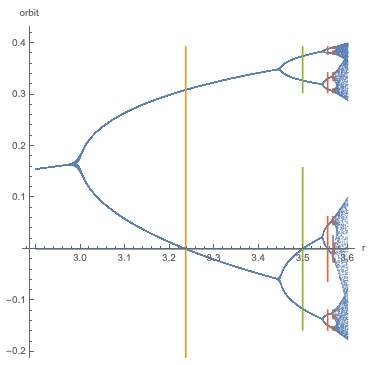
\includegraphics[width=0.45\textwidth]{img/191111-C28p1a.png}
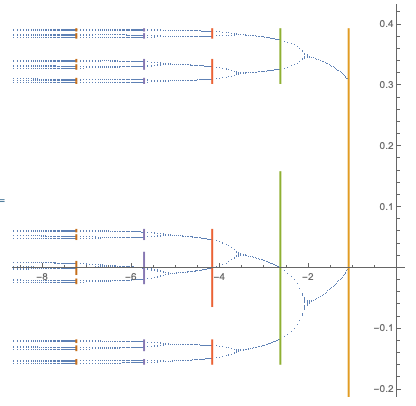
\includegraphics[width=0.45\textwidth]{img/191111-C28p1b.png}

On the left is the usual orbit diagram.  On the right, I am showing $r$ on a log scale based on the distance to $r_{\infty}$, the limiting $r$ value associated with the period-doubling cascade.

\vspace{0.2cm}
\hrule
\vspace{0.2cm}
\noindent\textbf{Your questions}
\begin{enumerate}
    \item Rossler attractor.
    \begin{enumerate}
    \item For the Rossler attractor, is Steve showing just one trajectory?
    \item Where do we see chaos with this attractor?
    \item How do the parts of the attractor connect?
    \item What is happening in the re-injection step?
    \end{enumerate}
    \item Fractals and dimension
    \begin{enumerate}
        \item How did we find the dimensions?
        \item How does the Cantor set relate to any of the other topics we have worked with?
        \item It is hard to think about the van Koch curve having infinite length.  What does its similarity dimension of $1.26$ mean?
    \end{enumerate}
    \item Do we see the Cantor set and stretching/folding in real-world systems?
\end{enumerate}

\vspace{0.2cm}
\hrule
\vspace{0.2cm}

\noindent\textbf{Skill Check C28 practice}
\begin{questions}
\item Retake of skill check C25.

\item Recall that the similarity dimension, $d$, is given by $m = r^d$ where $r$ is a scaling factor and $m$ is the number of copies.

Find the similarity dimension for the square-based Sierpinski gasket shown below.  

\emph{The points in the set are shown in blue: you're seeing its construction through four iterates of the process.}


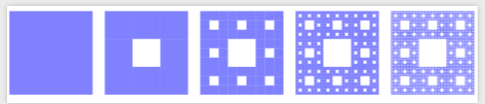
\includegraphics[width=\textwidth]{img/C29-2019-11-13p2.png}


\begin{tabular}{|c|p{3cm}|}
\hline
& \\
scaling factor: & $r =$ \\
& \\
\hline
& \\
copies: & $m=$ \\
& \\
\hline
& \\
dimension: & $d=$ \\
& \\
\hline
\end{tabular}

\end{questions}

\noindent\textbf{Skill Check C28 Practice Solution}

\vspace{0.1cm}

\begin{tabular}{|c|p{3cm}|}
\hline
scaling factor: & $r = 3$ \\
\hline
copies: & $m=8$ \\
\hline
dimension: & $d=\ln 8/\ln 3$ \\
\hline
\end{tabular}


\vspace{0.1cm}

From the left image to the second image, each side of the large square scales down by a factor of three, and then we make eight copies (we are leaving the center one out).  So the dimension should be almost $2$, but not quite.

$8 = 3^d$ so $d = \ln 8/\ln 3 \approx 1.89$.

\vspace{0.2cm}

\hrule
\vspace{0.2cm}


\noindent\textbf{Questions}

\noindent \ \ 0.  Share your favorite animal with your team, and write your names on the slide.

\begin{questions}

\question (The Rossler system.)

The Rossler equations are:
\begin{align*}
\dot x &= -y-z \\
\dot y &= x + a y \\
\dot z &= b + z(x-c)
\end{align*}

This is a slightly simpler system then the Lorenz system (and its dissipation / volume contraction is slower).


$a = 0.2, b=0.2,c=5$ is a parameter set associated with chaos.

\begin{parts}
\item Find the nonlinear term(s) in the system.  How many are there?
\item We map a `Lorenz map' for this system using local maximum values of $x(t)$ (it looks nicer than local maxima of $z(t)$).  I'll call it the `Rossler map'.  

On the left is a trajectory with those local maxima plotted on it as tiny red dots. On the right is the resulting map (for $c = 4.5$ in red and $c=5$ in blue).

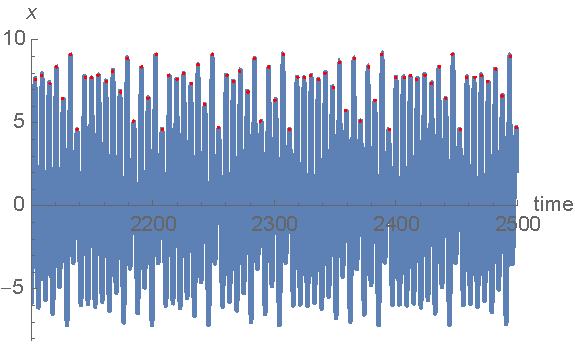
\includegraphics[scale=0.8]{img/191108-C27p5d.pdf}
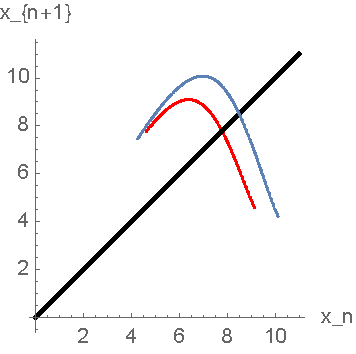
\includegraphics[scale=0.8]{img/191108-C27p5c.pdf}

Using a range of $c$ values and plotting those success maxima (so the orbit of the `Rossler map'), I have the following orbit diagram:

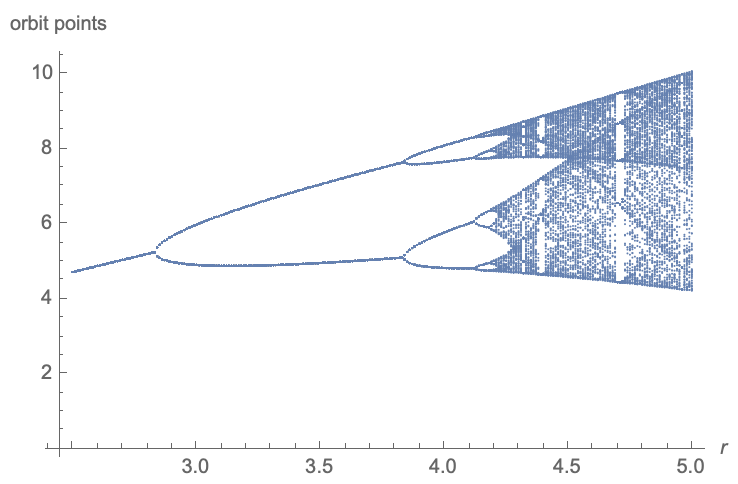
\includegraphics[scale=0.8]{img/191108-C27p5b.png}

What is it similar to?  Can you find a period-6 window? 

\emph{It looks like I didn't go to large enough $c$ for the obvious period-3 window to show up.}

\part Here are some trajectories of the Rossler system at various values of $c$.  You can hopefully see the periodic structures from the orbit diagram manifest as trajectories in phase space.

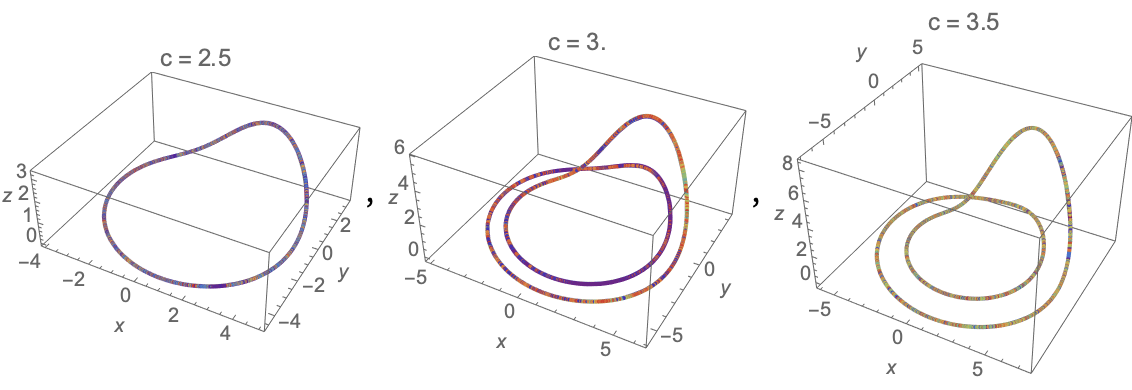
\includegraphics[width=0.7\textwidth]{img/191108-C27p5e.png}

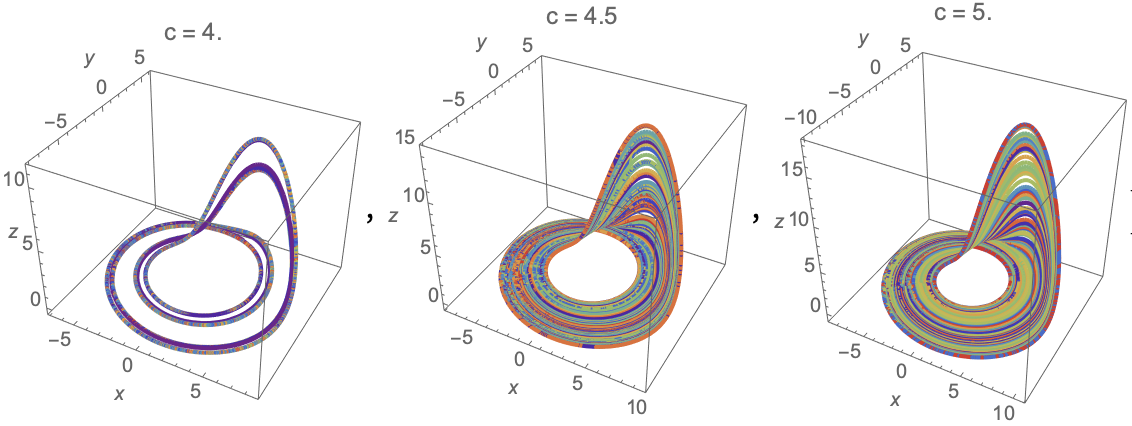
\includegraphics[width=0.7\textwidth]{img/191108-C27p5f.png}

What are the periods you see?  Which trajectories seem aperiodic?

\end{parts}

\question The middle-thirds Cantor set, $C$, is the set of points that remains in the interval $S_0 = [0,1]$ under the following procedure: 
\begin{itemize}
\item Remove the middle third of the interval (remove an open set, so that the endpoints remain behind).  This removes the interval $(1/3, 2/3)$.  The points that remain are the set $S_1$.
\item For every subinterval that is left in $[0,1]$, remove its middle third.  The points that remain are the set $S_2$. Then repeat this removal forever ($S_3, S_4, ... S_\infty)$.
\end{itemize}
The middle-thirds Cantor set, $C = S_\infty$, is the set of points that remains in $[0,1]$ when this procedure of removal is repeated indefinitely.
\begin{parts}
\item Sketch $S_0$, $S_1$, $S_2$, and $S_3$.
\item The Cantor set is a simple fractal and has self-similarity.  Convince yourself that the left third of $S_2$ looks like $S_1$ scaled down by $3$.  Similarly, the left third of $S_{k+1}$ looks like $S_{k}$ scaled down by $3$.  Finally, argue that the left third of $S_\infty$ is $S_\infty$ scaled down by $3$.
\item Add up the length of all of the line segments that you have removed as you formed the Cantor set.  Subtract this from $1$.  This will allow you to find the \emph{measure} of the Cantor set, the total length of the intervals left in the set.
\end{parts}

\question (Our first 2D map) 

The Baker's map is given by
\[B(x_n,y_n)= (x_{n+1},y_{n+1}) = \left\{ \begin{array}{c c} (2x_n, ay_n) &\mbox{ for } 0\leq x_n \leq \frac{1}{2} \\ (2x_n-1, ay_n+\frac{1}{2}) &\mbox{ for } \frac{1}{2} \leq x_n \leq 1 \end{array} \right. .\]  It is illustrated by Figure 12.1.4 of the text, shown below.

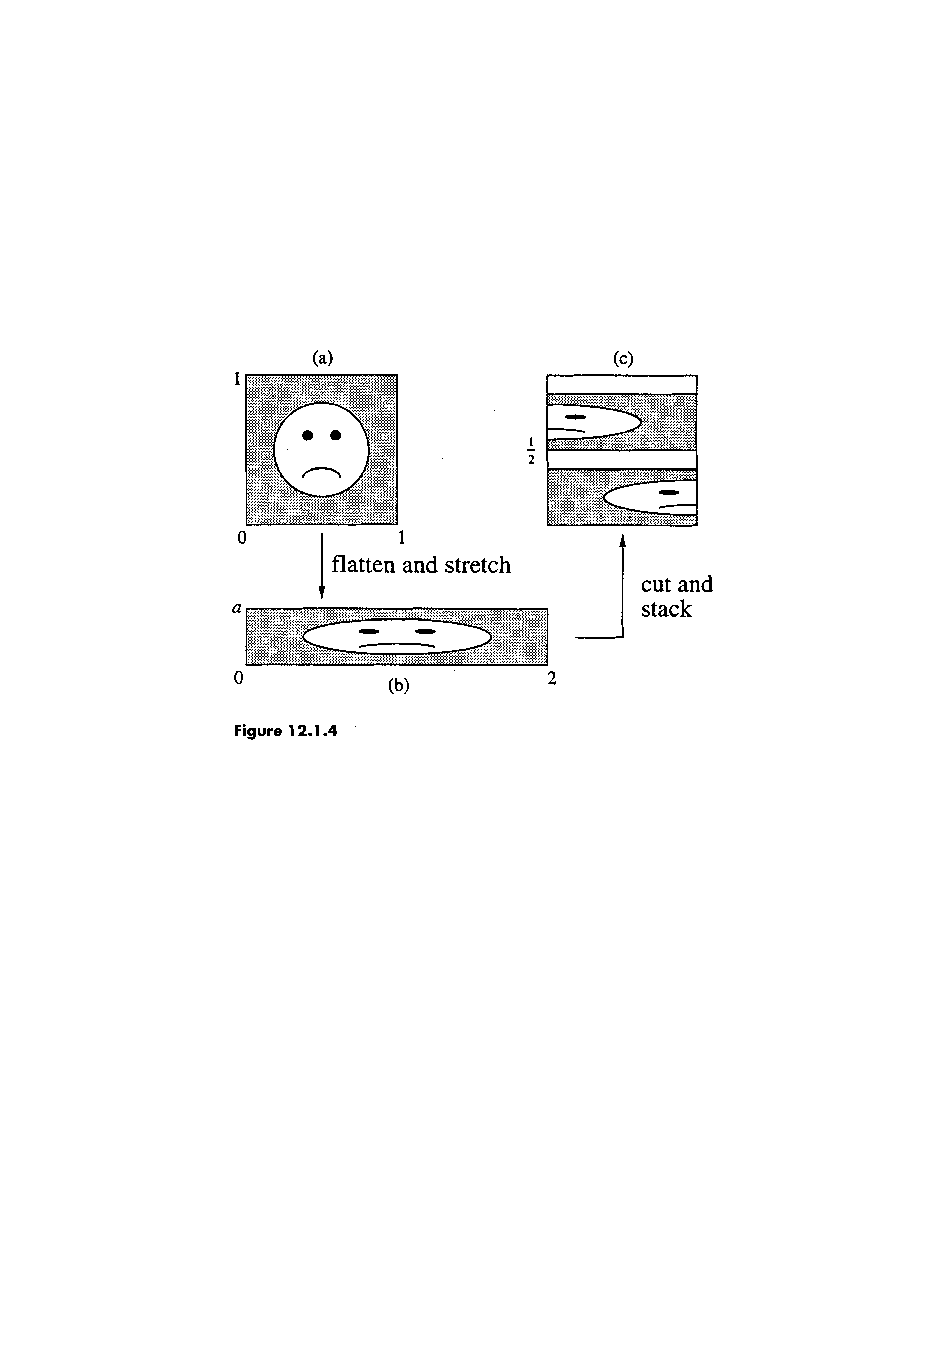
\includegraphics[scale=1]{img/C25baker.pdf}

The Baker's transformation is a simple model with chaotic dynamics.  We can reason about the long term behavior under this map by thinking geometrically, or by rewriting the map as a shift map on a sequence of numbers.

% This map can be expressed via \textbf{symbolic dynamics}, or dynamics that are represented via shifts on sequences of numbers.
\begin{parts}
\item $B(x_n, y_n)$ is equivalent to the procedure of stretching by $2$, flattening by $a$, then cutting and stacking, that is shown in the figure.  Convince yourself and your team that this is the case.  \emph{For $a<1/2$ there is are blank horizontal spaces present after stacking.  These are regions of the unit square that nothing in the original domain maps to.}
\item Sketch what will happen after one more iterate of the map shown in the figure.  \emph{Include the face and the bands of empty space (white space on this sheet)}.
\item This process might remind you of forming the Cantor set.  Sketch some representation of the limiting set.  How would you describe this set?   

\item Explain why we can't use similarity dimension to determine the dimension of the limiting set.
\item The box dimension is another way to compute fractal dimension.  Box dimension is given by
$d = \lim_{\epsilon \rightarrow 0} \frac{\ln N}{\ln \frac{1}{\epsilon}}$ where $N$ is the number of boxes needed to cover the set and $\epsilon$
is the side length of the boxes.  Compute the box dimension for the limiting set of the Baker's map.

\emph{Cover the $n^{th}$ iterate of the map with square boxes
of side length $a^n$.  Note that the first iterate has $2$ stripes and the second has $4$.  }
\item In the case $a = \frac{1}{2}$, your box dimension should be $2$ because the map is area preserving.  Check that this is the case.

\end{parts}


\end{questions}
\begin{enumerate}
\item
\begin{enumerate}
    \item There's one.  It is the $xz$ in the third equation.
    \item This looks like the logistic orbit diagram.  There is a visible period-6 window between $4.3$ and $4.4$.
    \item $c=2.5$: period-1.  $c = 3$: period-2.  $c=3.5$: period 2.  $c = 4$: I am seeing four, I think, so period 4 (and I confirmed that by looking at the orbit diagram).  $c= 4.5$ and $c=5$: look aperiodic.
\end{enumerate}


\item
\begin{enumerate}
 \item For the unit square, consider the sets \[S_0=\{(x,y): 0\leq x < \frac{1}{2}, 0\leq y < 1\}\]
 and \[S_1=\{(x,y): \frac{1}{2} \leq x < 1, 0\leq y < 1\}.\]  These are right half ($S_1$) and the left half ($S_0$) of the unit square.
 
 Under the action of the map, points in $S_0$ are mapped to $(2x, ay)$.  This stretches $S_0$ in the $x$ direction, by a factor of two so that it takes up the whole range $0\leq x < 1$.  In addition, $y$ is squished by a factor of $a$.  This is the same thing as what happens to $S_0$
 if we stretch by $2$, flatten by $a$, and then cut halfway across, as $S_0$ is not impacted by the cut/stack step of the procedure.

$S_1$ is also stretched and flattened.  The $(\frac{1}{2},0)$ corner of $S_1$
 is placed at $(0, \frac{1}{2})$, setting the placement of the whole stretched/flattened set.  This is also equivalent to
 what happens to the set $S_1$ under the flattening/stretching and cutting/stacking procedure shown in the image.
 \item 
 
 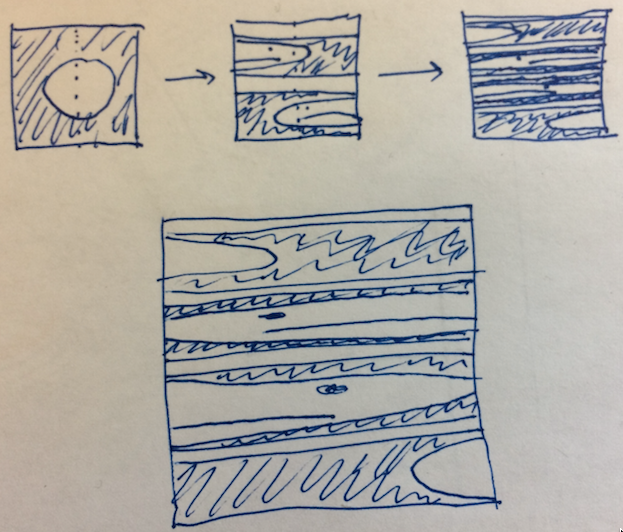
\includegraphics[width=4in]{img/C22bakers.png}
 
 \item The limiting set is like a Cantor set cross a line segment (so stripes spaced like a Cantor set).  Its dimension should be approximately $1+$ the dimension of the Cantor set, because it has an extra dimension.  \item The set isn't self similar: the length never changes, just the width shrinks. Similarity dimension doesn't make sense here.
 \item At the nth iterate, we have $2^n$ stripes and need $\frac{1}{a^n}$ boxes to cover a single stripe (stripes are of width $a^n$ and of length $1$), so there
 are $\left(\frac{2}{a}\right)^n$ boxes being used and the box size is $a^n$.  
 $d = \lim_{n\rightarrow\infty} \frac{\left(\frac{2}{a}\right)^n}{\ln \frac{1}{a^n}} = 1- \frac{\ln 2}{\ln a} = 1+ \frac{\ln 2}{\ln (1/a)}.$
 \item If we plug in $a = \frac{1}{2}$ we have $d = 1+ \frac{\ln 2}{\ln 2} = 2$.
 \end{enumerate}
\end{enumerate}

\end{document}